\documentclass{beamer}

%Rajouter les slides de photoélasticité à fin

%%%%%%%%%%%%%%%%%%%%%%%%%%%%%
% Tikz packages and settings
%%%%%%%%%%%%%%%%%%%%%%%%%%%%%

\usepackage{tikz}
\usepackage{pgfplots}
\usepackage{tikz-3dplot}
\pgfplotsset{compat=1.11}

\usetikzlibrary{shapes.geometric,calc,intersections}
\usetikzlibrary{shapes.arrows}
\usetikzlibrary{shadings}
\usetikzlibrary{patterns}
\usetikzlibrary{decorations.pathmorphing}
\usetikzlibrary{decorations.pathreplacing}


\usetikzlibrary{external}
\tikzset{external/aux in dpth={false}}
\tikzset{external/up to date check={simple}}
\tikzset{external/optimize command away={\includetexgraphics}{2}}

\tikzset{>=stealth}

%%%%%%%%%%%%%%%%%%%%%%%%%%%%%%%%%%%%%%%%%%%%%%%%%%%%%%%%%%%%
% Custom macro to input a tikz picture and setting its name
%%%%%%%%%%%%%%%%%%%%%%%%%%%%%%%%%%%%%%%%%%%%%%%%%%%%%%%%%%%%

\makeatletter
\newcommand{\includetikzgraphics}[1]{
	\filename@parse{#1}
	\tikzsetnextfilename{\filename@base}
	\input{#1}
}
\makeatother

%%%%%%%%%%%%%%%%%%%%%%%%%%%%%%%%%%
% Custom tikz command for drawing
%%%%%%%%%%%%%%%%%%%%%%%%%%%%%%%%%%

\tikzset{math3d/.style=
    {z= {(-0cm,-0.3cm)}, y={(0cm,1cm)},x={(1cm,0cm)}}}

% \drawYNema {x} {y} {yAngle}
\newcommand{\drawYnema}[3] {
	\shade [ball color=black] (#1,#2) ellipse 
		[x radius={sqrt(pow(cos(#3)*0.1,2)+pow(sin(#3)*0.3,2))}, y radius=0.1];
}
% \drawXNema {x} {y} {xAngle}
\newcommand{\drawXnema}[3] {
	\shade [ball color=black] (#1,#2) ellipse 
		[y radius={sqrt(pow(cos(#3)*0.1,2)+pow(sin(#3)*0.3,2))}, x radius=0.1];
}
% \drawZNema {x} {y} {zAngle}
\newcommand{\drawZnema}[3] {
	\shade [ball color=black] (#1,#2) ellipse 
		[x radius=0.3, y radius=0.1, rotate={#3}];
}

% \plotcylinder { radius } { heigth } { altitude }
\newcommand{\plotcylinder}[3] {
     \draw [math3d, fill=white, samples=100]
        plot[domain=-pi:pi] ({#1*cos(\x r)},#3,{#1*sin(\x r)}) ;
     \draw [math3d, fill=white, samples=100]
        plot[domain=0:pi] ({#1*cos(\x r)},#3,{#1*sin(\x r)}) --
        plot[domain=pi:0] ({#1*cos(\x r)},{#3-#2},{#1*sin(\x r)}) --
        cycle;
}

% \plotpolarizer { x} { y} { z } { radius } { angle }
\newcommand{\plotpolarizer}[5] {
    \draw [math3d, fill=gray, opacity=0.8, samples=100]
        plot[domain=-pi:pi] ({#1+#4*cos(\x r)},#2,{#3+#4*sin(\x r)}) ;
    \draw [math3d, opacity=0.8]
        ({#1+#4*cos(#5)},#2,{#3+#4*sin(#5)}) -- ({#1-#4*cos(#5)},#2,{#3-#4*sin(#5)}) ;
}

% \fancyarrow {xi} {yi} {xf} {yf} {width} {options}
\newcommand{\fancyarrow}[6]{
	\pgfmathsetmacro{\dx}{#3-#1};
	\pgfmathsetmacro{\dy}{#4-#2};
	\pgfmathsetmacro{\dl}{sqrt(\dx*\dx+\dy*\dy)};
	\pgfmathsetmacro{\dw}{#5/2};
	\pgfmathsetmacro{\cos}{\dx/\dl};
	\pgfmathsetmacro{\sin}{\dy/\dl};
	\draw [#6] (#1,#2) -- ++($\dw*(\sin,-\cos)$) 
		-- ++(${\dl-2*\dw}*(\cos,\sin)$)
		-- ++($\dw*(\sin,-\cos)$) -- ++($2*\dw*(\cos,\sin)+2*\dw*(-\sin,\cos)$) 
		-- ++($-2*\dw*(\cos,\sin)+2*\dw*(-\sin,\cos)$) -- ++($\dw*(\sin,-\cos)$)
		-- ++(${2*\dw-\dl}*(\cos,\sin)$) -- cycle;
}

%%%%%%%%%%%%%%%%%%%%%%%
% Custom pgf mark list
%%%%%%%%%%%%%%%%%%%%%%%
\pgfplotscreateplotcyclelist{colorhollowmarks}{%
	{black,mark=x},
	{cyan,mark=+},
	{magenta,mark=o},
	{teal,mark=square},
	{violet,mark=triangle},
	{gray,mark=diamond},
	{brown,mark=pentagon},
	{orange,mark=otimes},
	{lime,mark=10-pointed star}}
\pgfplotscreateplotcyclelist{hollowmarks}{%
	{mark=x},
	{mark=+},
	{mark=o},
	{mark=square},
	{mark=triangle},
	{mark=diamond},
	{mark=pentagona},
	{mark=otimes},
	{mark=10-pointed star}}
\pgfplotscreateplotcyclelist{onlycolors}{%
	black,
	cyan,
	magenta,
	teal,
	violet,
	lightgray,
	brown,
	orange,
	lime}


\usepackage[utf8]{inputenc}
\usepackage[english]{babel}
\usepackage{amsmath}
\usepackage{animate}
\usepackage[absolute,overlay]{textpos}
\usepackage{animate}
\usepackage{graphicx}
\usepackage{stmaryrd}
\usepackage{ulem}

\everymath{\displaystyle}

\usepackage{bm}
\setbeamertemplate{navigation symbols}{}
\setbeamercolor{structure}{fg=red!30!black}

\usetheme{Warsaw}
\setbeamertemplate{headline}{}
\addtobeamertemplate{footline}{\ \ \ \ \ \insertframenumber/\inserttotalframenumber\hspace{2em}\null}

\title{Chauffage par impact des planétésimaux}
\author{Félix Bunel et Hadrien Vergnet}
\titlegraphic{
\includegraphics[height=1.7cm]{figures/sdm.png} 
\includegraphics[height=1.5cm]{figures/geol.jpg}} 
\date{12/12/2016}

\usefonttheme[onlymath]{serif}

%%%%%%%%%%%%%%%%%%%%%%%%%%%%%%%%%%%%%%%%%%%%%%%%%%%%%%%%%%%%%%%%%%%%%%%%%%%%%%%%%%%%%
\begin{document}
%%%%%%%%%%%%%%%%%%%%%%%%%%%%%%%%%%%%%%%%%%%%%%%%%%%%%%%%%%%%%%%%%%%%%%%%%%%%%%%%%%%%%

%%%%%%%%%%%%% Slide de garde
\begin{frame}[plain]

\begin{columns}
\begin{column}{3.3cm}
\center
   
\includegraphics[height=1.3cm]{figures/logo_lyon1.jpg}
\end{column}
\begin{column}{3.3cm}
\center

\includegraphics[height=1.3cm]{figures/logo_ens.jpg}
\end{column}
\begin{column}{3.3cm}
\center

\includegraphics[height=1.3cm]{figures/logo_univ_lyon.jpg}
\end{column}
\end{columns}

\titlepage
\end{frame}
%%%%%%%%%%%%%

\title{Chauffage par impact des planétésimaux}
%%%%%%%%%%%%%
\begin{frame}
\frametitle{Introduction}
\framesubtitle{\ }

\begin{center}
 \Large Comment un noyau peut-il se former rapidement ?
\end{center}

\begin{itemize}
\item La séparation des métaux des silicates se fait sous forme (partiellement) fondue.
\end{itemize}

\begin{center}
 \Large D'où vient l'énergie nécessaire à la fusion ?
\end{center}

\begin{textblock*}{5cm}(0.5cm,4.5cm) % {block width} (coords)
	\center
	\begin{itemize}
		\item Chauffage radioactif
	\end{itemize}
	\vspace{0.1cm}
	
    
\includegraphics[width = 2cm]{figures/radioactif.png}
\end{textblock*}

\begin{textblock*}{5cm}(7.5cm,4.5cm) % {block width} (coords)
	\center
	\begin{itemize}
		\item Chauffage par impact
	\end{itemize}
	
	\vspace{0.1cm}
    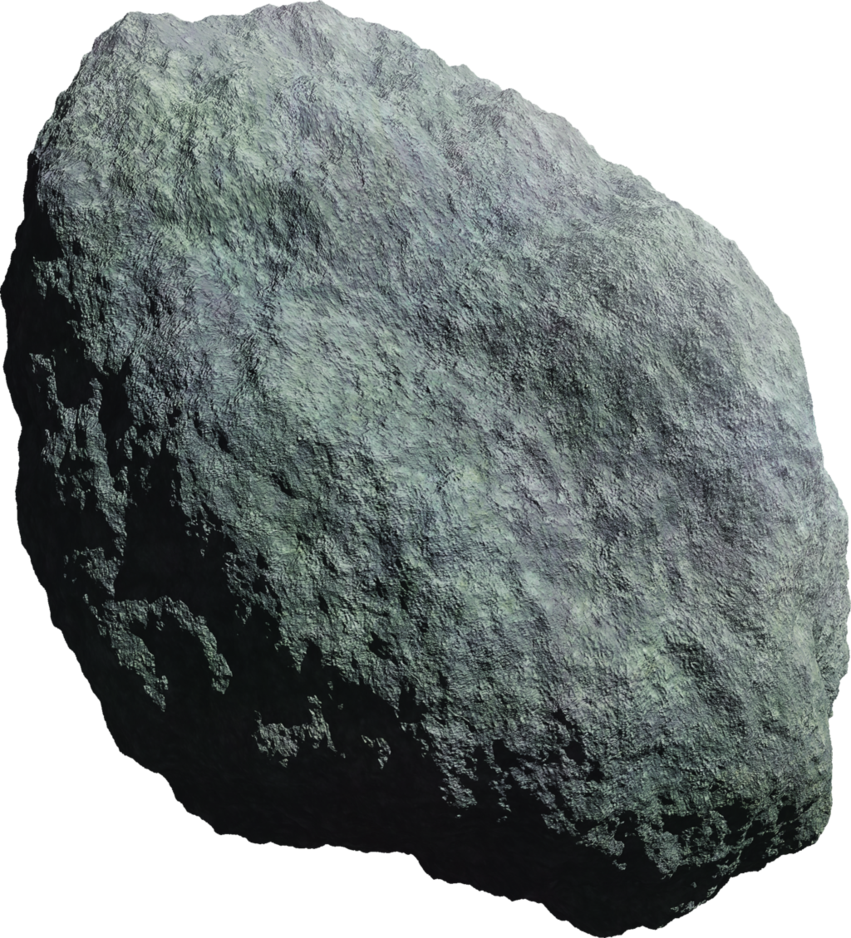
\includegraphics[width = 2cm]{figures/asteroid.png}
\end{textblock*}

\center
\vspace{1cm}
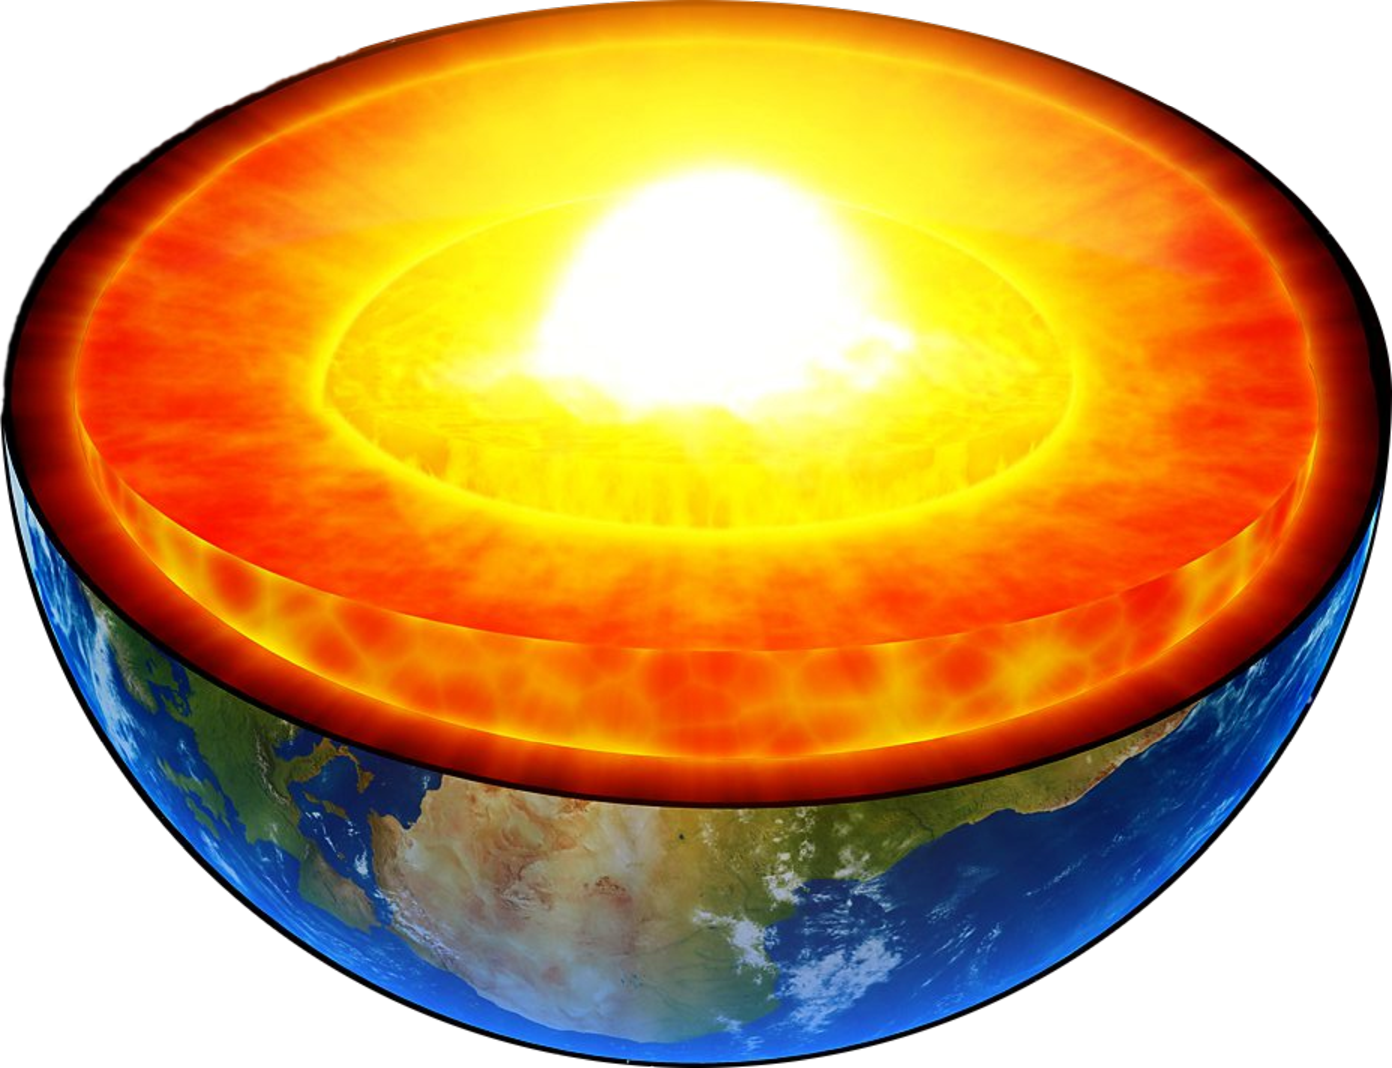
\includegraphics[width = 4cm]{figures/terre_core.pdf}

\end{frame}
%%%%%%%%%%%%%


%%%%%%%%%%%%% Slide de sommaire
\begin{frame}
	\frametitle{Sommaire}
	\framesubtitle{\ }
	\tableofcontents
\end{frame}
%%%%%%%%%%%%%

\section{Un problème de diffusion}
\subsection{Equation de la diffusion}

%%%%%%%%%%%%% 
\begin{frame}
	\frametitle{Un problème de diffusion}
	\framesubtitle{Equation de la diffusion}

{\Large
$$\rho C_p \dfrac{\partial T}{\partial t}= k_{T} \Delta T  + P$$
}
\begin{columns}
    \begin{column}{6cm}
      \center {\Large + }{\large perte radiative\\ à la surface}
	\end{column}

	\begin{column}{6cm}
      \center {\Large + }{\large chaleur latente\\ de changement d'état}
	\end{column}
\end{columns}

\begin{columns}
    \begin{column}{6cm}      
	  \center 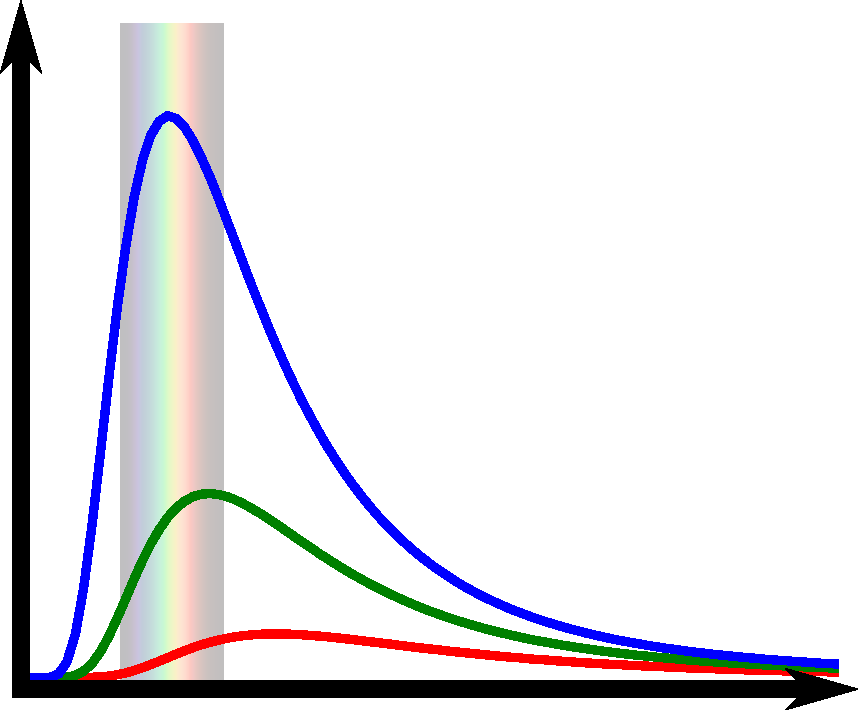
\includegraphics[width = 5cm]{figures/blackbody.pdf}  
	\end{column}

	\begin{column}{6cm}     
      \center 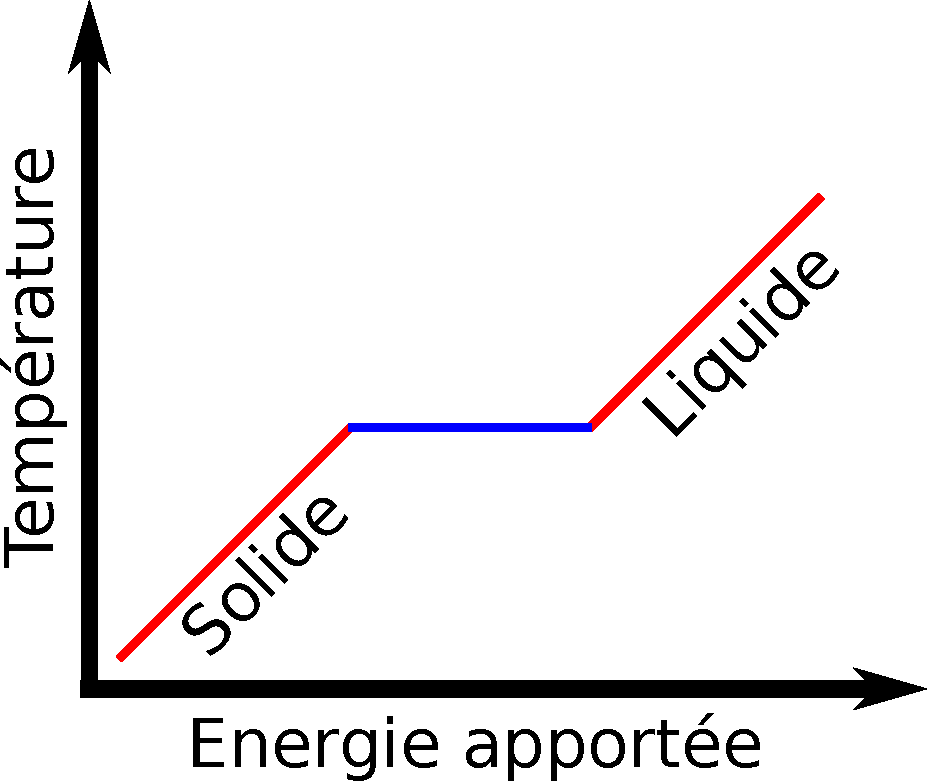
\includegraphics[width = 5cm]{figures/lattentheat.pdf}
      \vspace{-0.4cm}
      
	\end{column}
\end{columns}

\end{frame}
%%%%%%%%%%%%%

\subsection{Grandeurs caractéristiques}

%%%%%%%%%%%%% 
\begin{frame}
	\frametitle{Un problème de diffusion}
	\framesubtitle{Grandeurs caractéristiques}
	

\begin{columns}
    \begin{column}{4cm}
      \center 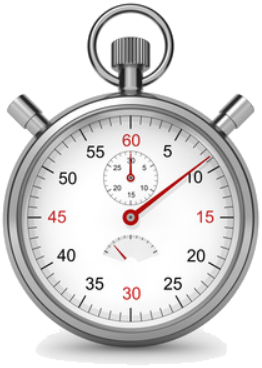
\includegraphics[height =  2cm]{figures/chrono.png}
	\end{column}

	\begin{column}{4cm}
      \center 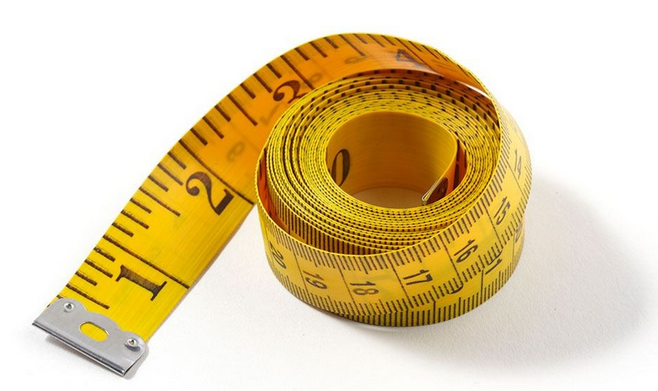
\includegraphics[height = 2cm]{figures/ruban.png}
	\end{column}
	
	\begin{column}{4cm}
      \center 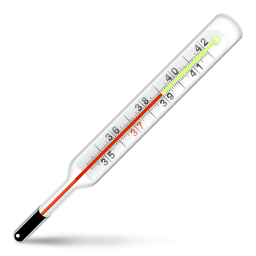
\includegraphics[height = 2cm]{figures/thermo.png}
	\end{column}
\end{columns}

\vspace{0.5cm}

\begin{columns}
    \begin{column}{4cm}
      \center
      Temps de demi-vie
	\end{column}

	\begin{column}{4cm}
      \center
      Longueur de diffusion 
	\end{column}
	
	\begin{column}{4cm}
      \center
      Température de la nébuleuse
	\end{column}
\end{columns}

\vspace{0.5cm}

\begin{columns}
    \begin{column}{4cm}
      $$\tau_{1/2}$$
	\end{column}

	\begin{column}{4cm}
      $$\sqrt{\dfrac{k_T\tau_{1/2}}{\rho C_p}}$$
	\end{column}
	
	\begin{column}{4cm}
      $$T_{neb}$$     
	\end{column}
\end{columns}

\vspace{0.5cm}

\begin{columns}
    \begin{column}{4cm}
      $$\simeq 0.7 \text{ My}$$
	\end{column}

	\begin{column}{4cm}
      $$\simeq 10\text{ km}$$
	\end{column}
	
	\begin{column}{4cm}
      $$\simeq 300 \text{ K}$$       
	\end{column}
\end{columns}
	
\end{frame}
%%%%%%%%%%%%%

\subsection{Condition initiale}

%%%%%%%%%%%%% 
\begin{frame}
	\frametitle{Un problème de diffusion}
	\framesubtitle{Condition initiale}

\vspace{-1cm}

\begin{columns}
    \begin{column}{7cm}      
	  \center 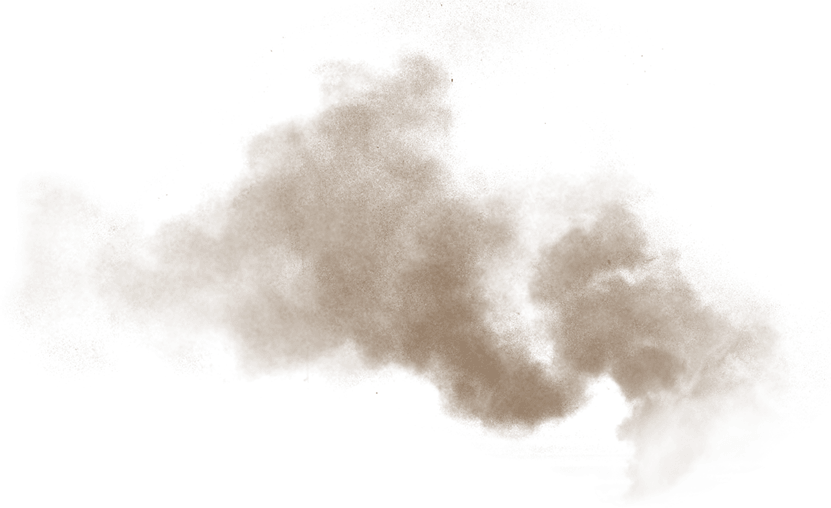
\includegraphics[height = 4cm]{figures/dust.png}  
	\end{column}
	
	\begin{column}{1cm}      
	  \center {\huge $\Rightarrow$}  
	\end{column}

	\begin{column}{5cm}     
      \center 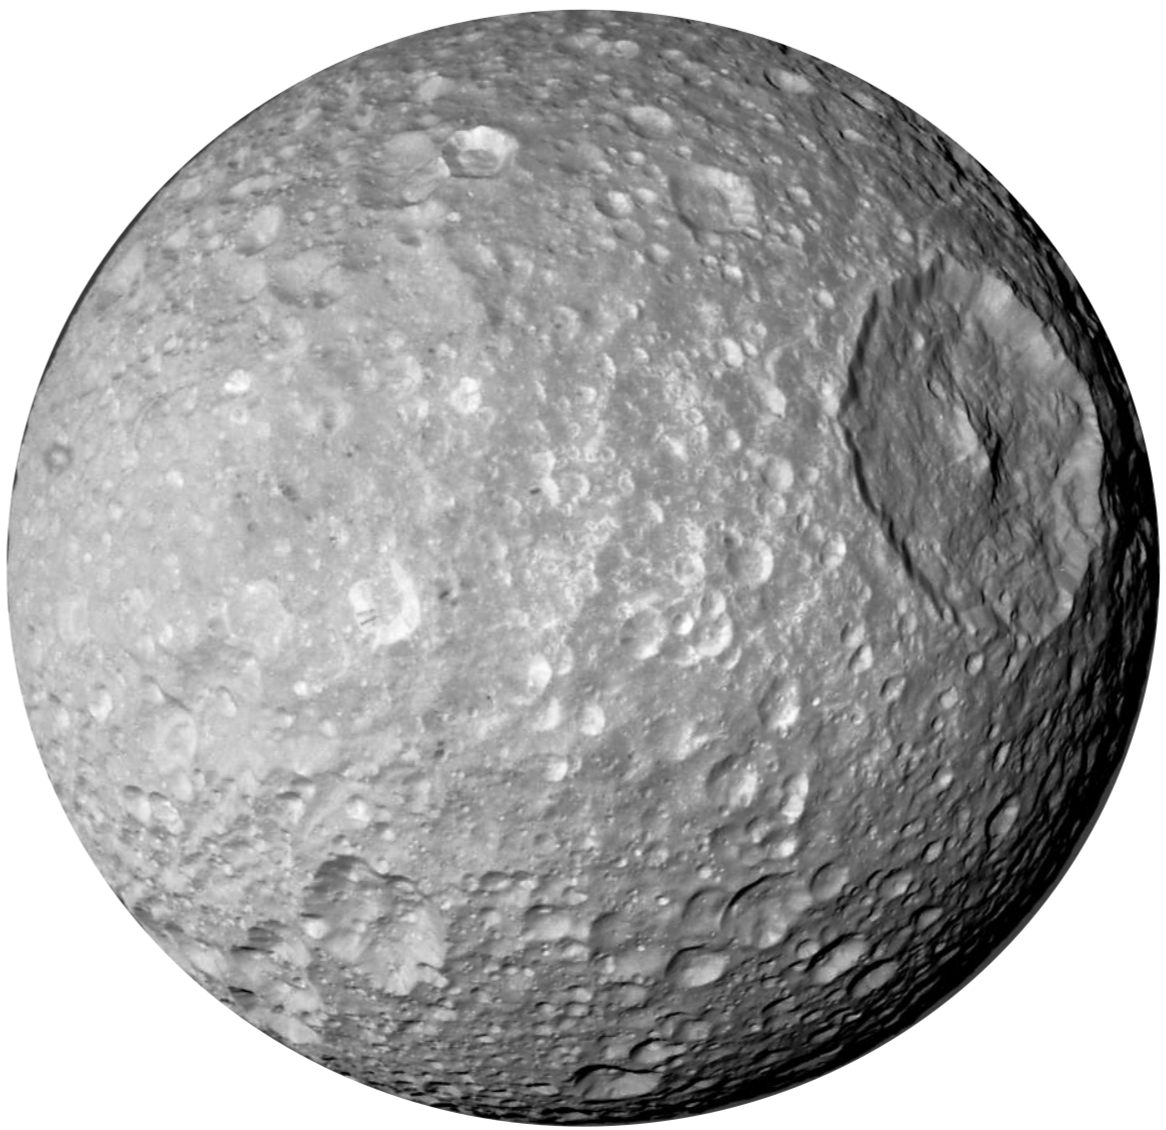
\includegraphics[width = 3cm]{figures/mimas.png}
      \vspace{-0.4cm}
	\end{column}
\end{columns}

\center
Accrétion rapide d'un nuage de poussière en planétésimal.
\vspace{0.5cm}

$\rightarrow$ L'énergie gravitationnelle $ E = \dfrac{3}{5} \dfrac{GM^2}{R}$ est convertie en chaleur.

$$T^0 \ =\  T_{neb} + \frac{4\pi}{5}\frac{\rho G}{C_p} R^2 \  \simeq \ T_{neb}$$

\end{frame}
%%%%%%%%%%%%%

\subsection{Méthodes numériques}

%%%%%%%%%%%%% 
\begin{frame}
	\frametitle{Un problème de diffusion}
	\framesubtitle{Discrétisation}
	

Spatiale : $T(r) \rightarrow T_i$ 
$$\Delta T = \frac{T_{i+1} + T_{i-1} - 2T_{i}}{\Delta r ^2} $$ 


Temporelle : $T(t) \rightarrow T^i$ 
$$\dfrac{\partial T}{\partial t} = \frac{T^{i+1}-T^{i}}{\Delta t} $$


$$\rho C_p \dfrac{\partial T}{\partial t}= k_{T} \Delta T  + P
\quad \sim \quad (Id + M) T^{i+1}=T^i + P$$


$$
M =
\begin{bmatrix}
    2      & -1     & -1        &      &     \\
    -1      &  2     & -1        &     &              \\
     & \ddots & \ddots    & \ddots &       \\
 &     &  -1      &  2     & -1                      \\
     &    &    -1      & -1     & 2          
\end{bmatrix}
$$

\end{frame}
%%%%%%%%%%%%%

\section{Chauffage radioactif}
\subsection{Influence de la taille du planétésimal}

%%%%%%%%%%%%% 
\begin{frame}
	\frametitle{Chauffage radioactif}
	\framesubtitle{Influence de la taille du planétésimal}
\vspace{-0.5cm}

\center 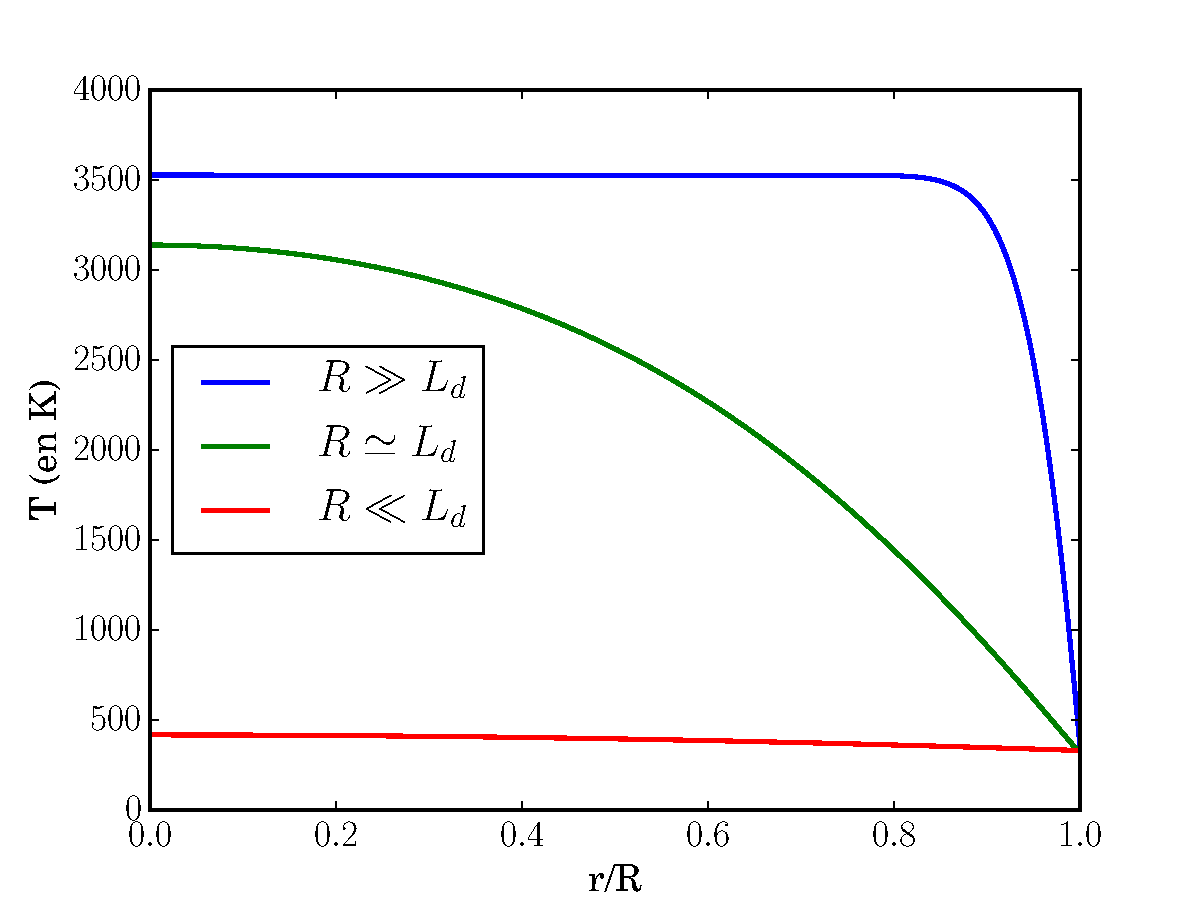
\includegraphics[width = 9cm]{figures/diffusion2.pdf} 
 
Profil de température après 1 million d'années pour différents $R$.


	  	
\end{frame}
%%%%%%%%%%%%%

\subsection{Influence de la chaleur latente}

%%%%%%%%%%%%% 
\begin{frame}
	\frametitle{Chauffage radioactif}
	\framesubtitle{Influence de la chaleur latente}
\vspace{-0.5cm}

\center 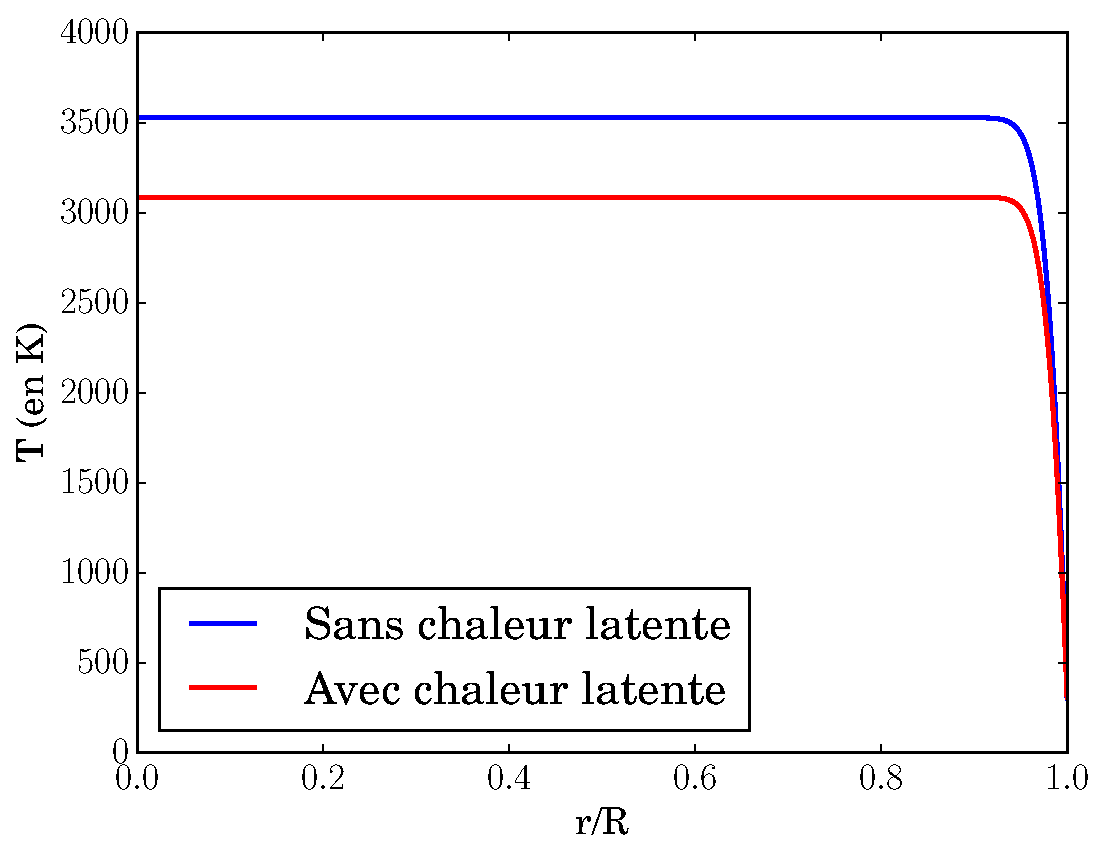
\includegraphics[width = 9cm]{figures/diffusion1.pdf}
  
Profil de température après 1 million d'années pour $R = 500$ km.
	  	
\end{frame}
%%%%%%%%%%%%%



\subsection{Evolution en température}

%%%%%%%%%%%%% 
\begin{frame}
	\frametitle{Chauffage radioactif}
	\framesubtitle{Evolution de la température}
\vspace{-0.5cm}

\center 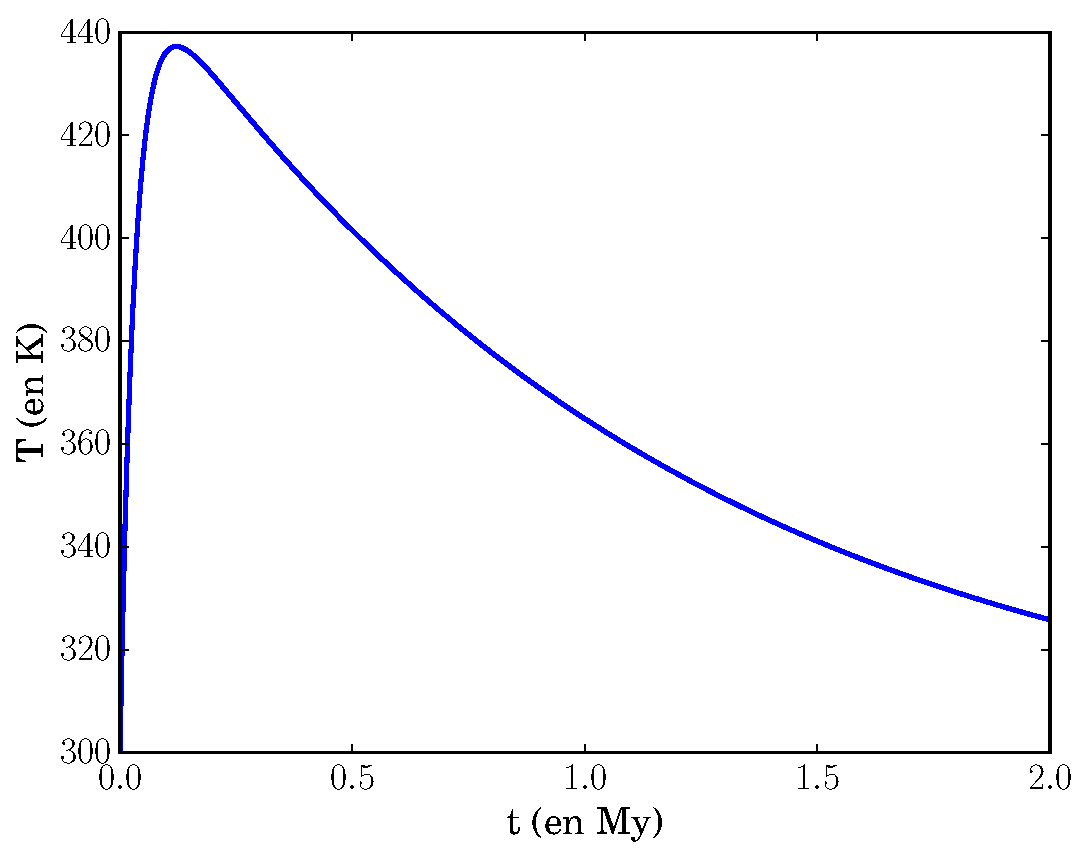
\includegraphics[width = 9cm]{figures/tempMoy.pdf}  

Température moyenne en fonction du temps pour $R = 5$ km.
	  	
\end{frame}
%%%%%%%%%%%%%

\section{Ajout d'un terme d'accrétion}
\subsection{Evolution du rayon}

%%%%%%%%%%%%% 
\begin{frame}
	\frametitle{Ajout d'un terme d'accrétion}
	\framesubtitle{Evolution du rayon}

		{\Large $$\rho C_p \left(\dfrac{\partial T}{\partial t} - \dot{R}\dfrac{\partial T}{\partial R}\right)  = k_{T} \Delta T  + P$$}
\begin{columns}
    \begin{column}{3.7cm}
      	{\huge $$\ \ \dot{R} \simeq R^\beta$$}
      	$5\rightarrow500$ km en 1 My
	\end{column}

	\begin{column}{9cm}
\center 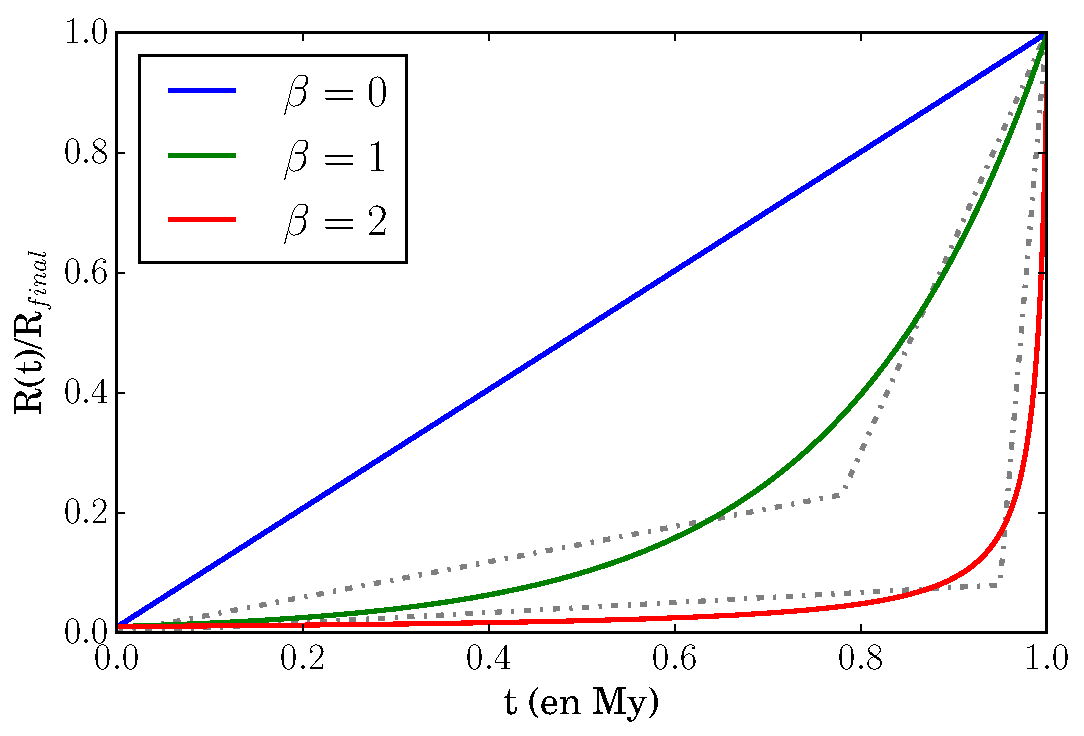
\includegraphics[width = 8.5cm]{figures/rayon.pdf}
	\end{column}
\end{columns}
\end{frame}
%%%%%%%%%%%%%

\subsection{Profil de température}

%%%%%%%%%%%%% 
\begin{frame}
	\frametitle{Ajout d'un terme d'accrétion}
	\framesubtitle{Profil de température}
\vspace{-0.5cm}

\center 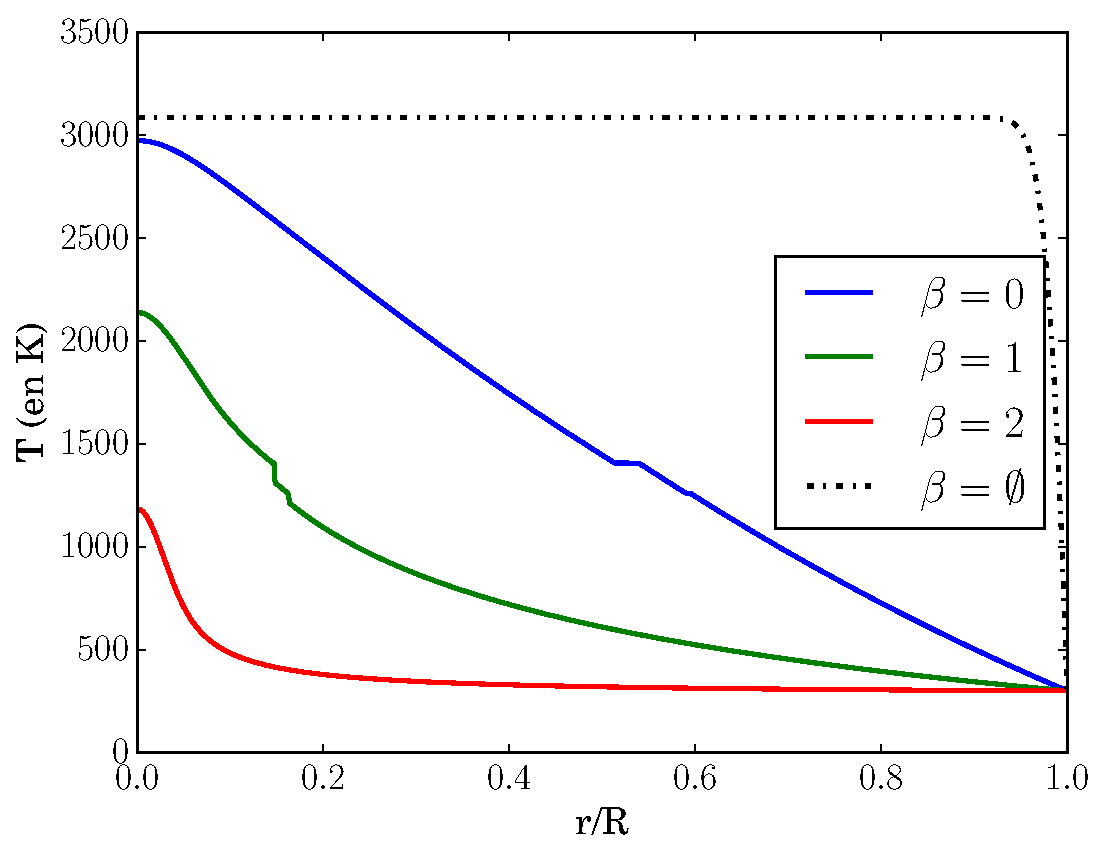
\includegraphics[width = 9cm]{figures/profil_acre.pdf} 
 
Profil de température après 1 million d'années pour $R = 500$ km.
	  	
\end{frame}
%%%%%%%%%%%%%

\subsection{Influence sur les températures}
%%%%%%%%%%%%% 
\begin{frame}
	\frametitle{Ajout d'un terme d'accrétion}
	\framesubtitle{Evolution de la température}

\center 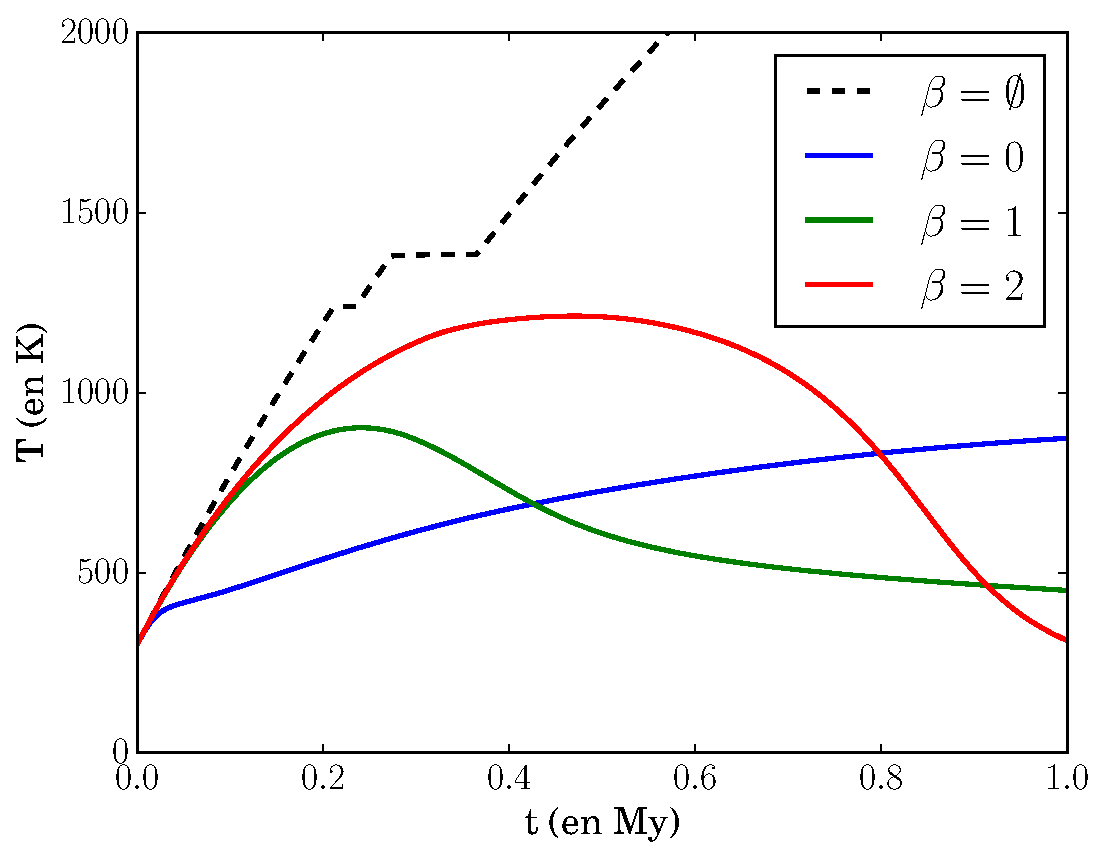
\includegraphics[width = 9cm]{figures/tempMoy_acretion.pdf}

Température moyenne en fonction du temps.

\end{frame}
%%%%%%%%%%%%%

\section{Chauffage par impact}
\subsection{Description du modèle}

%%%%%%%%%%%%% 
\begin{frame}
	\frametitle{Chauffage par impact}
	\framesubtitle{Description du modèle}
	
\vspace{-0.3cm}
\center 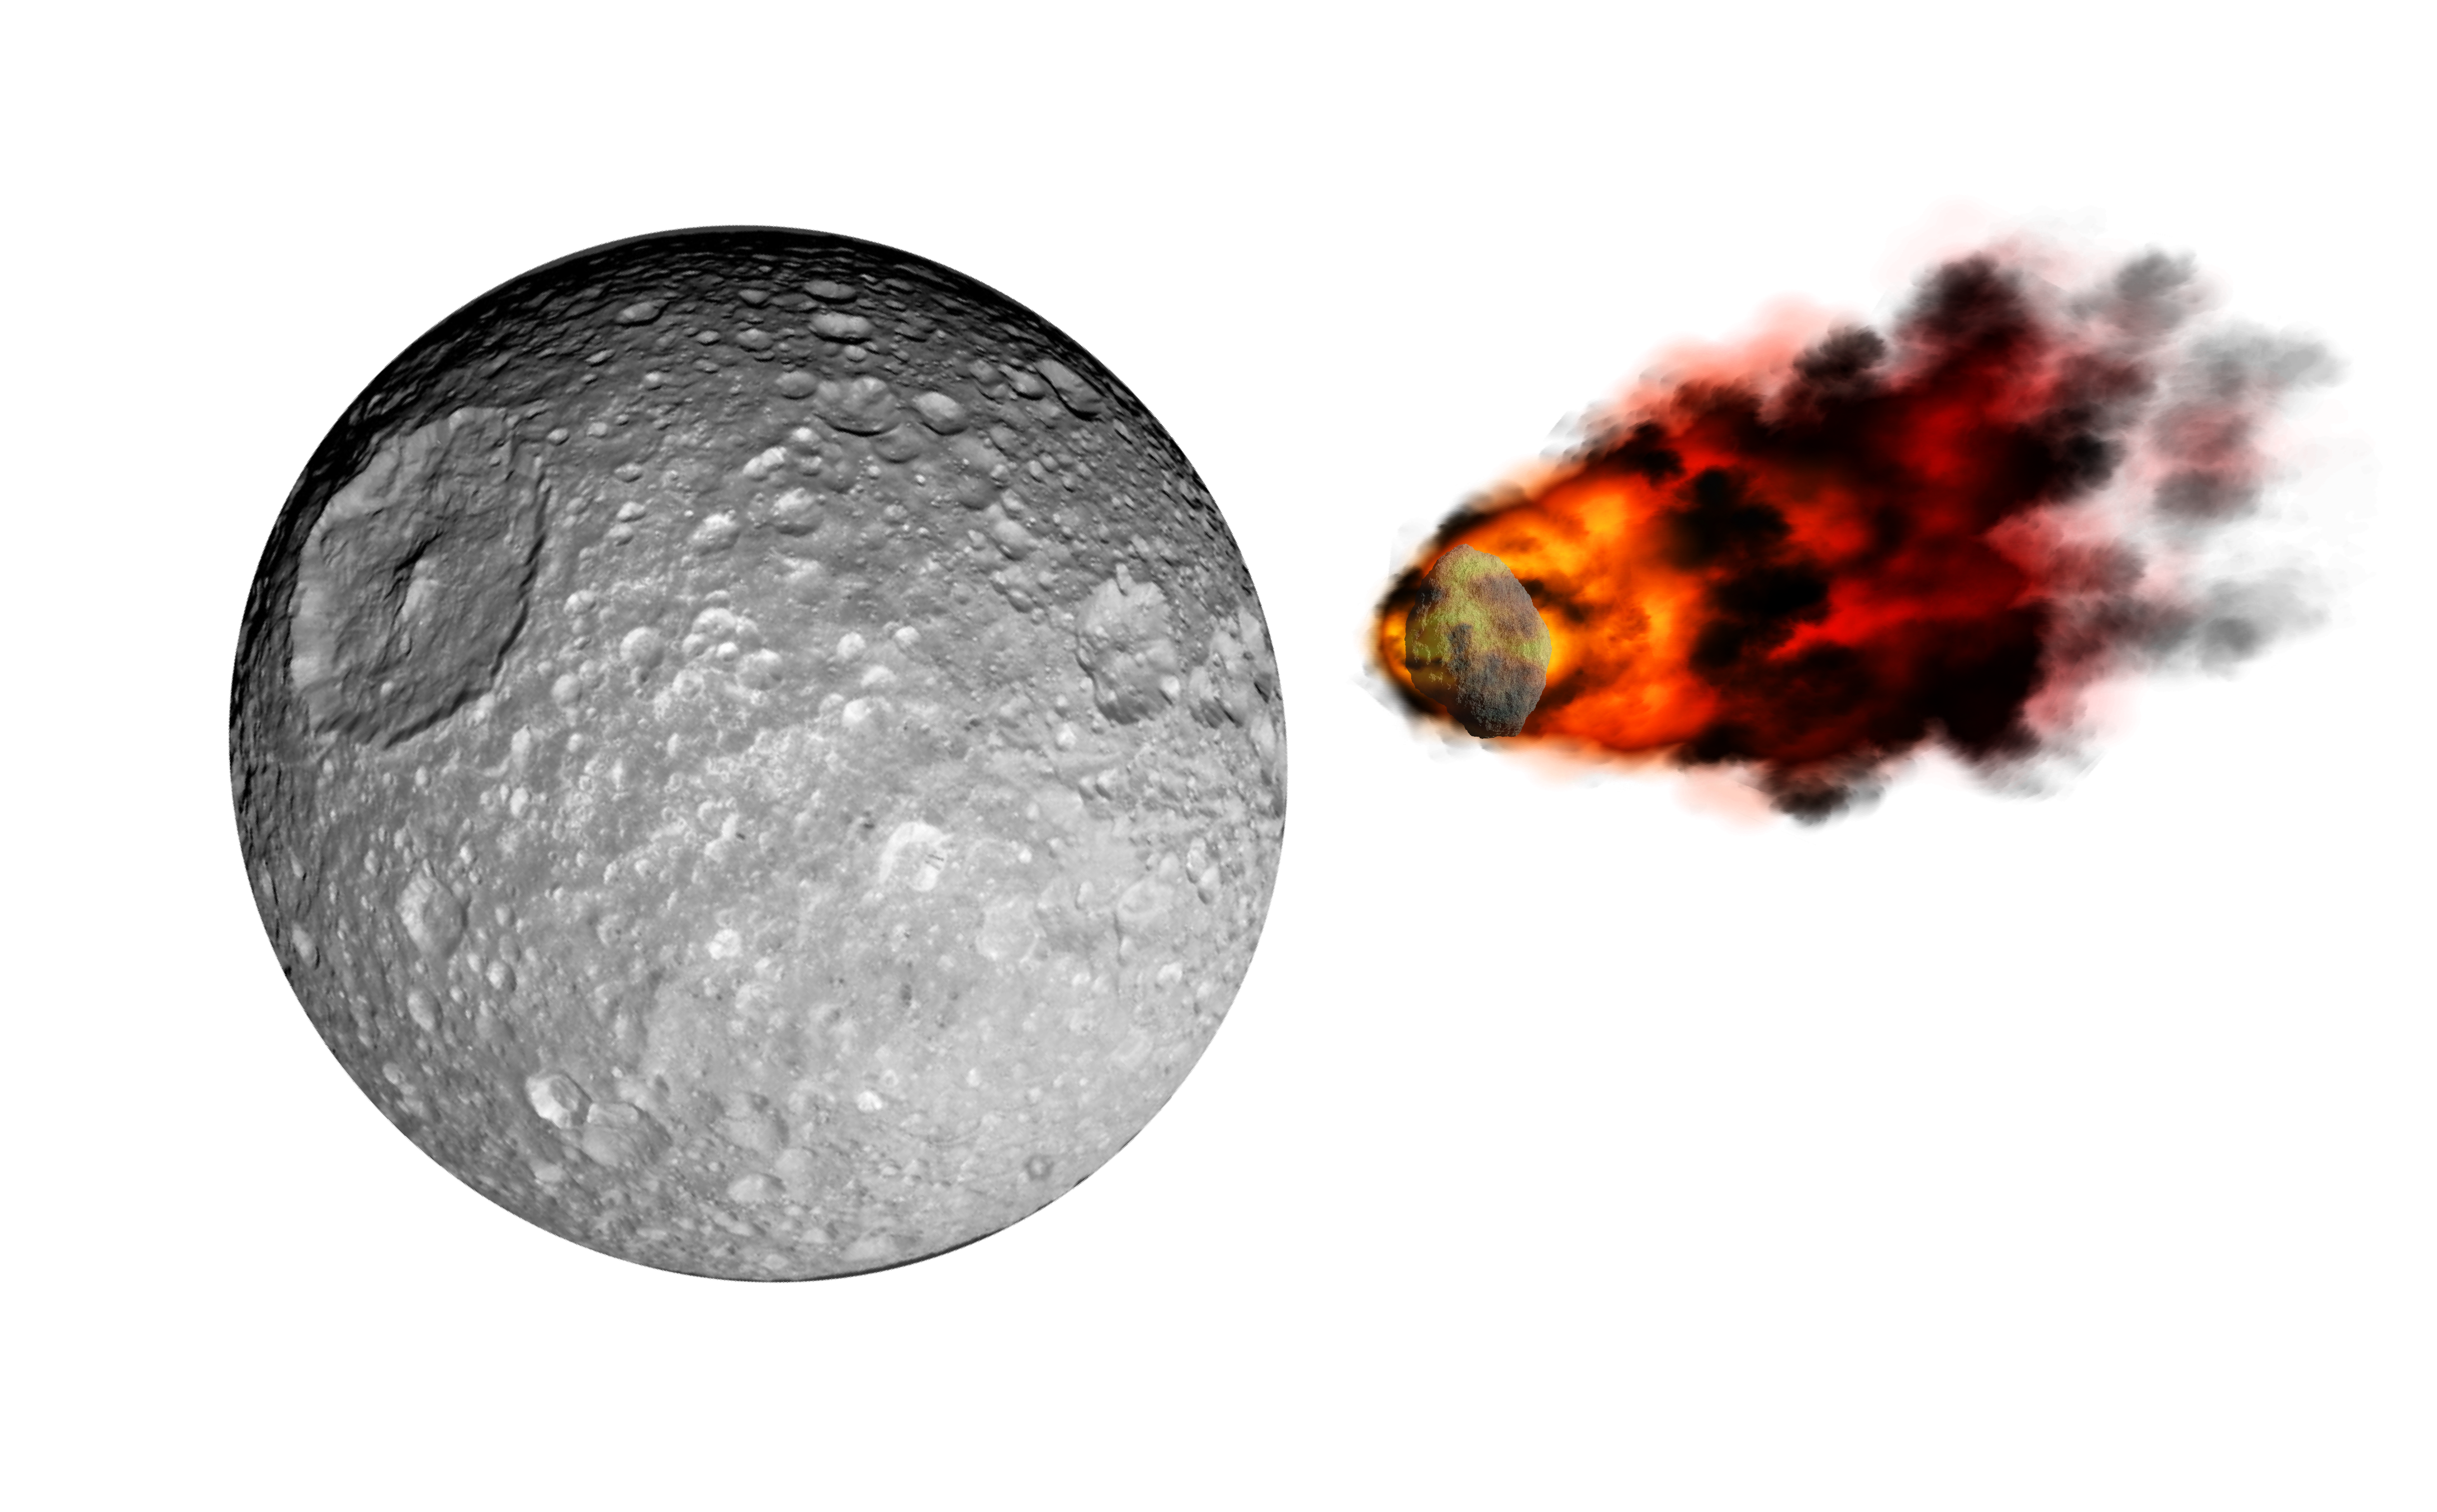
\includegraphics[height = 5cm]{figures/impact.pdf}  

\vspace{-0.5cm}
Energie des impactants : 

énergie gravitationnelle + énergie thermique
\vspace{0.3cm}

\begin{enumerate}
\item La croissance est due à la masse apportée par les impactants
\item Seulement $20\%$ de l'énergie des impactants est introduite
\item L'énergie est répartie sur une couche d'épaisseur $R/5$
\item La température des impactants est de 1000 K 
\end{enumerate}
\end{frame}
%%%%%%%%%%%%%

\subsection{Profil de température}

%%%%%%%%%%%%% 
\begin{frame}
	\frametitle{Ajout d'un terme d'accrétion}
	\framesubtitle{Profil de température}
\vspace{-0.5cm}

\center 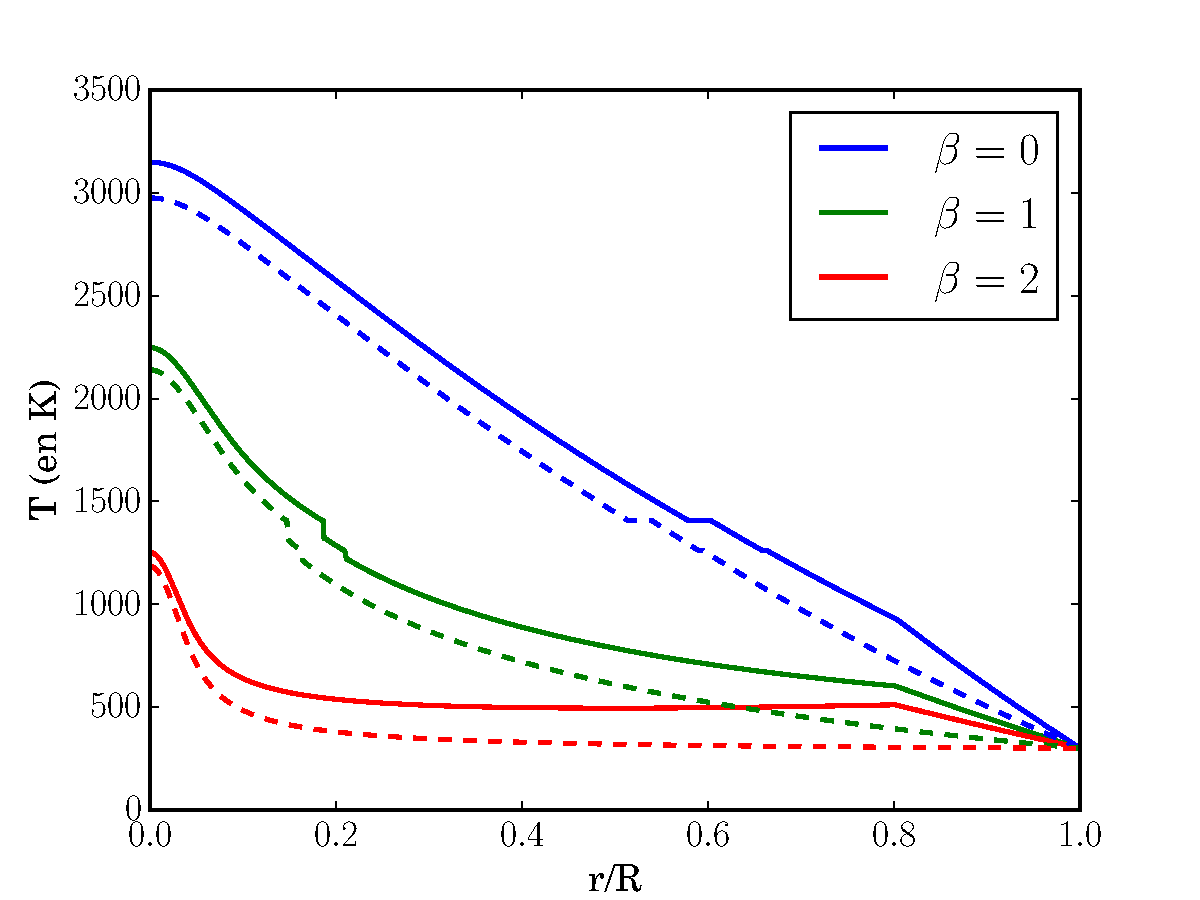
\includegraphics[width = 9cm]{figures/profil_acre_impact.pdf} 
 
Profil de température après 1 million d'années pour $R = 500$ km.
	  	
\end{frame}
%%%%%%%%%%%%%

%%%%%%%%%%%%% 
\begin{frame}
	\frametitle{Conclusion}
	\framesubtitle{\ }
	


\begin{itemize}
\item L'énergie apportée par l'impact n'est pas très importante dans la formation du noyau.
\vspace{0.5cm}

\item Le noyau n'apparaît que pour une croissance rapide au début de la vie du planétésimal ($\beta = 0$ et $\beta = 1$).
\end{itemize}




	
\end{frame}
%%%%%%%%%%%%%

%%%%%%%%%%%%% 
\begin{frame}
	\frametitle{Perspectives}
	\framesubtitle{\ }
\begin{itemize}
\item 
\begin{enumerate}
\setcounter{enumi}{3}
\item \sout{La température des impactants est de 1000 K}

$\rightarrow$ La température des impactants est calculée




\center 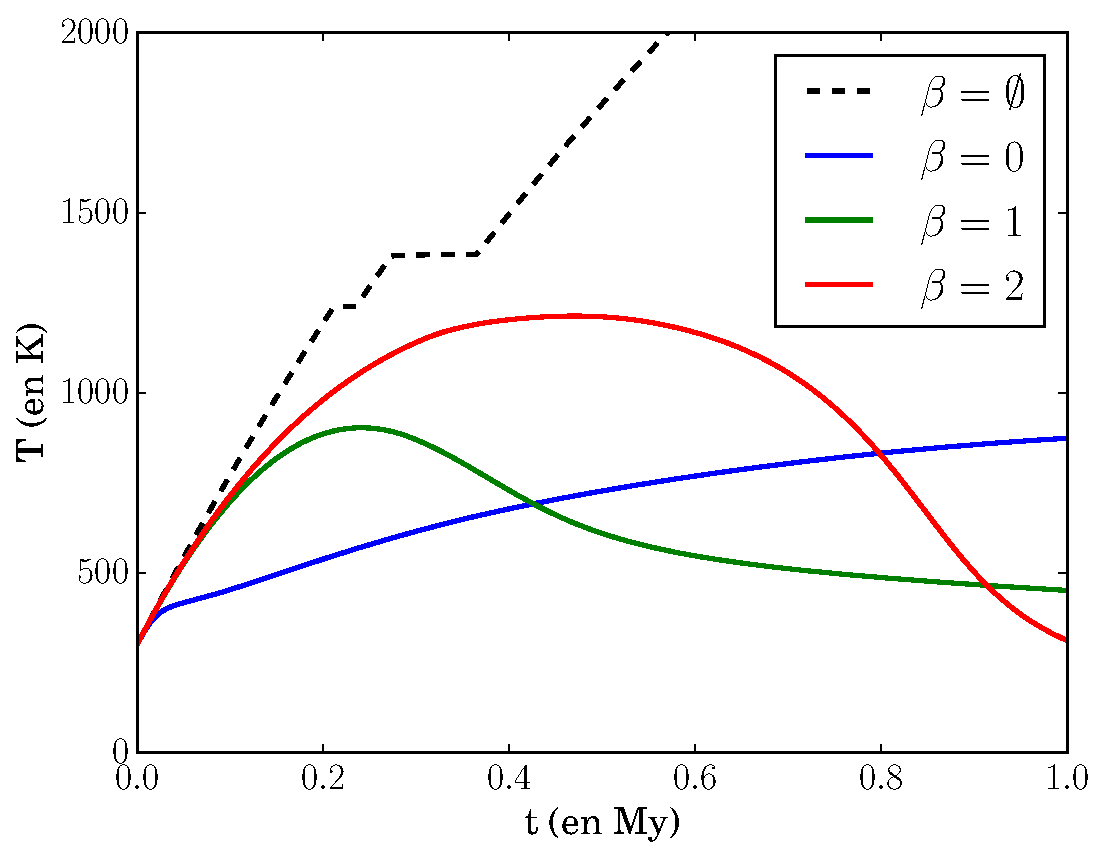
\includegraphics[width = 3cm]{figures/tempMoy_acretion.pdf}
\vspace{-0.45cm}

\center \scalebox{.3}{Température moyenne en fonction du temps.}

\end{enumerate}
\item Influence de la vitesse des impacts sur le surplus de température.
\item Séparation métal-silicate :

\center 
\includegraphics[width = 3cm]{figures/phaseseparation.pdf}

$\rightarrow$ La séparation favorise la formation d'un noyau


\end{itemize}
\end{frame}
%%%%%%%%%%%%%

%%%%%%%%%%%%% 
\begin{frame}
	\frametitle{\ }
	\framesubtitle{\ }

{\center $\qquad$ \Huge Merci pour votre attention}

\end{frame}
%%%%%%%%%%%%%

%%%%%%%%%%%%% 
\begin{frame}
	\frametitle{Equation matricielle}
	\framesubtitle{\ }
	
$$
(Id + M)T^{t+1} = T^t + c_0 ( P + S )
$$	
	
$$c_0 = \frac{\Delta t \tau_{1/2} }{\rho C_p T_{neb}}$$ 

$$
M = \frac{\Delta t ~ r^2_{i+1/2}}{r^2_i \Delta r^2} ~ d1 + \frac{\Delta t ~ r^2_{i-1/2}}{r^2_i \Delta r^2} ~ d2  
$$

$$
d1=
\begin{bmatrix}
    2      & -1     & -1       &   \\
           &  1     & -1              &             \\
     &        & \ddots    &\ddots       \\
     &        &            & 1 & -1         \\
         &   &      &   0         &  0
\end{bmatrix}
d2=
\begin{bmatrix}
     0     & 0      &   &     &        \\
    -1     & 1      &  &          &            \\
     & \ddots & \ddots &    &      \\
     &              &  -1      &  1         \\
         &      &  -1     & -1        & 2 \\
\end{bmatrix}
$$

\end{frame}
%%%%%%%%%%%%%


%%%%%%%%%%%%%
\end{document}